\documentclass[tikz,border=3pt]{standalone}
\usepackage[utf8]{inputenc}
\usepackage[T1]{fontenc}
\usepackage{lmodern}
\renewcommand{\familydefault}{\sfdefault}
\usepackage{sansmath}\sansmath
\usepackage{chemfig}
\usepackage{pgfplots}\pgfplotsset{compat=1.18,/pgf/number format/use comma,/pgf/number format/1000 sep={.}}
\usetikzlibrary{arrows.meta,calc,positioning,decorations.pathmorphing,patterns}
% paleta del sitio
\definecolor{nar}{HTML}{E8680C}\definecolor{narc}{HTML}{FFB35C}\definecolor{hielo}{HTML}{FFF3E8}
\definecolor{tinta}{HTML}{1D1D1F}\definecolor{gris}{HTML}{6E6E73}\definecolor{lila}{HTML}{7C5CF0}
\definecolor{azul}{HTML}{2F6FD6}\definecolor{menta}{HTML}{17A673}\definecolor{coral}{HTML}{E8342A}
\begin{document}
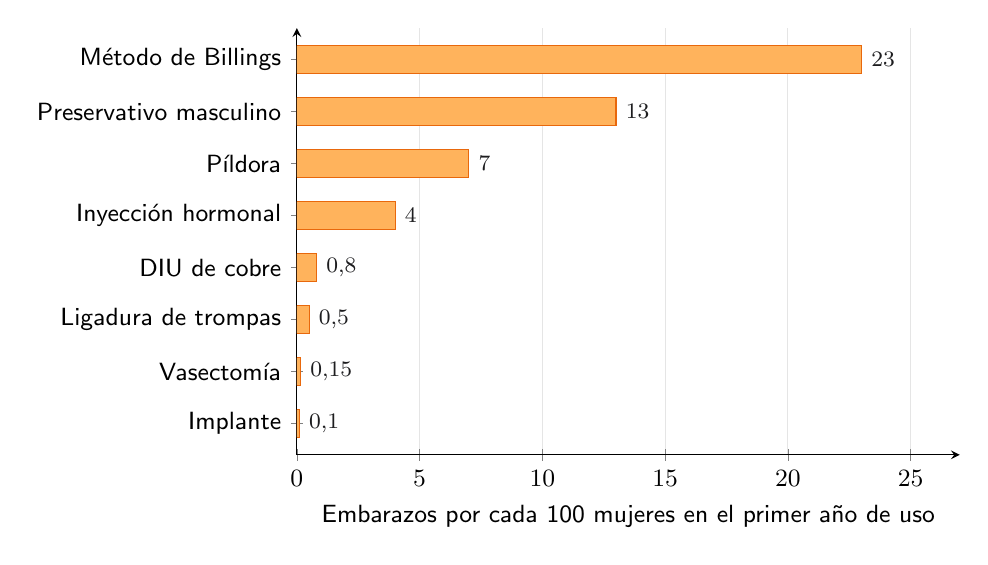
\begin{tikzpicture}[font=\small]
\begin{axis}[width=10cm,height=7cm,xbar,bar width=10pt,xmin=0,xmax=27,ymin=0.4,ymax=8.6,axis lines=left,
 ytick={1,...,8},yticklabels={Implante,Vasectomía,Ligadura de trompas,DIU de cobre,Inyección hormonal,Píldora,Preservativo masculino,Método de Billings},
 xlabel={Embarazos por cada 100 mujeres en el primer año de uso},xmajorgrids,grid style={gray!20},
 nodes near coords,every node near coord/.append style={font=\footnotesize,text=tinta},
 /pgf/number format/precision=2]
\addplot[fill=narc,draw=nar] coordinates {(0.1,1)(0.15,2)(0.5,3)(0.8,4)(4,5)(7,6)(13,7)(23,8)};
\end{axis}
\end{tikzpicture}
\end{document}
